\chapter{Problem with the Concurrent Analysis Method}

The analysis technique presented in the previous chapter, propagates the data flow values across inter-thread edges in the same way as it propagates the data flow along intra-thread edges. Consider the output of heap-liveness analysis technique on the same example of the previous chapter. The figure 5.1 is the final data flow value obtained after convergence. \\

	\begin{figure}
		\centering
		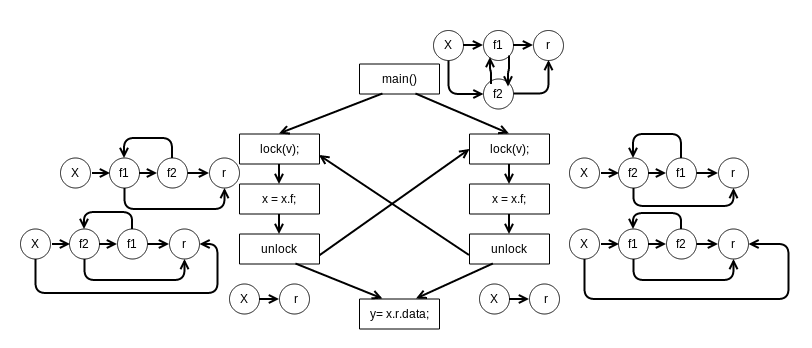
\includegraphics[width=0.8\textwidth]{Figures/conc_analysis_itr4.png}
		\caption{Example of the concurrent analysis technique}
		\label{fig:ch5example}
	\end{figure}


At the program point containing the main statement, the possible live links would be \emph{x.f1.f2.r} or \emph{x.f2.f1.r}. However the final data flow value  obtained at the main statement includes access links \emph{x.f1.r}, \emph{x.f2.r} , \emph {x.\{f2.f1\}\textsuperscript{+}.r}, \emph{x.\{f1.f2\}\textsuperscript{+}.r} which are imprecise values. The major source of error is due to no bound on the number of transitions from node $f_1$ to $f_2$ and from $f_2$ to $f_1$ in the access graph. \\

The imprecise data flow values are a result of taking into account execution of critical sections more than once. The thread synchronization edges introduce loops in the program graph. The current method treats these thread synchronization edges as loops and continues propagation of the facts until a converged value is obtained (as seen in the previous chapter). \\

\section{Execution of Critical Sections}

The execution of a multi-threaded program is an interleaving of statements of the multiple threads. Critical sections are regions where the shared variables are accessed under mutual exclusion. Note that addition of synchronization edges leads to formation of loop in the control flow graph. Due to this, data flow value is transferred to every critical section multiple times(even if there was no loop around the critical section before adding the synchronization edges).  Thus there is a need to identify the critical sections that only execute once. The analysis to figure this out is thread independent. Note that a critical section can only be executed once if there are no backward program edges from a statement after unlock(v) to one before lock(v) in the thread. For such critical sections we need to keep track to thread switches encountered while performing the analysis. In the example figure 5.1, if the critical section of thread 1 is analyzed and the data flow value is transferred to thread 2 for analysis along an inter-thread edge, it is required to ensure that data flow value in not transferred back to thread 1 after analysis of thread 2 critical section. \\


For handling such cases, we need to examine the presence of loops within each thread. 
\begin{itemize}
	\item If there is no loop within and across a critical section, it can only be executed once.
	\item If a loop is present within a critical section, even then the critical section can be executed only once. This is so because if 1 thread enters a critical section, all other threads wait until the this thread completes executing the loop inside the critical section.
	\item It a loop is present across a critical section in a thread, then the critical section can be executed zero or more number of times. Apart from that we may have execution of other critical sections between two executions on this critical section (inter-leaving) possible.
\end{itemize} 

Thus we need to figure out how to store the thread switchings in an access graph. One possible way is to store thread id corresponding to every edge in the access graph. Once each edge is labeled, we need to identify which paths are possible with respect to the execution semantics. For instance, as pointed above, we cannot allow paths with multiple thread switches into a critical section which can only be executed once. We will now need to examine all the paths where the execution semantics are followed. \\

\section{Examples highlighting the problems}

\begin{figure}
	\centering
	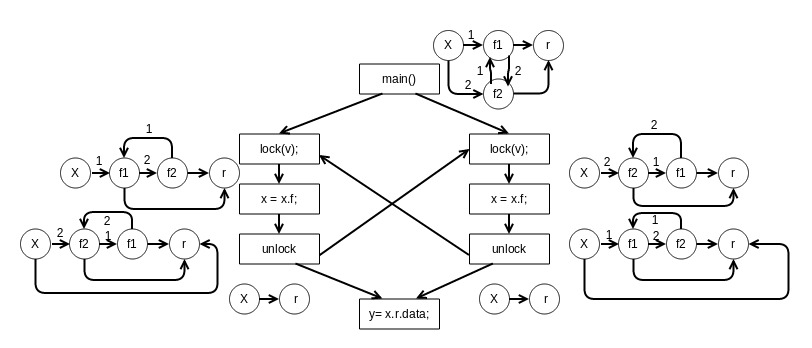
\includegraphics[width=0.8\textwidth]{Figures/conc_analysis_thr_itr3.jpg}
	\caption{Concurrent Heap liveness analysis example. Note that edges are marked by thread id}
	\label{fig:threadidanalysis}
\end{figure}

In figure 5.2, at the point main, we obtain an access graph which includes multiple access links. By imposing the restrictions that concurrent sections in thread 1 and 2 can only be executed once, we can discard all the access paths that contain more than 1 edges labeled 1 or 2. This way we can ensure that we get precise links. \\

Suppose we take another example in which we have an inner loop in a critical section (see figure 5.3). The access  graph obtained in this example is again similar to the previous example. The difference being that the loop in $thread_2$'s critical section can be executed zero or more times. Due to this we get an edge from $f2$ to itself in each of the final access graphs. Note however that  The possible executions of the program are either \emph{C1.C2\textsuperscript{*} } or \emph{ C2\textsuperscript{*}.C1 } , where $C_1$ and $C_2$ are critical sections of thread 1 and 2 respectively. Even in this example, applying the basic concurrent analysis shows access links that are not live to be live. For example links like {$x$.$f_1$.$f_2$\textsuperscript{*}.$f_1$}, which contain multiple occurrences of $f_1$. \\

For ensuring that only live paths are returned, we would need to impose the condition that critical section of thread 1 and thread 2 can only be executed once, while performing the analysis. We can allow 0 or more occurrence of edges labeled 2 whereas the number of edges labeled 1 must strictly be 1 for the example. \\ 

\begin{figure}
	\centering
	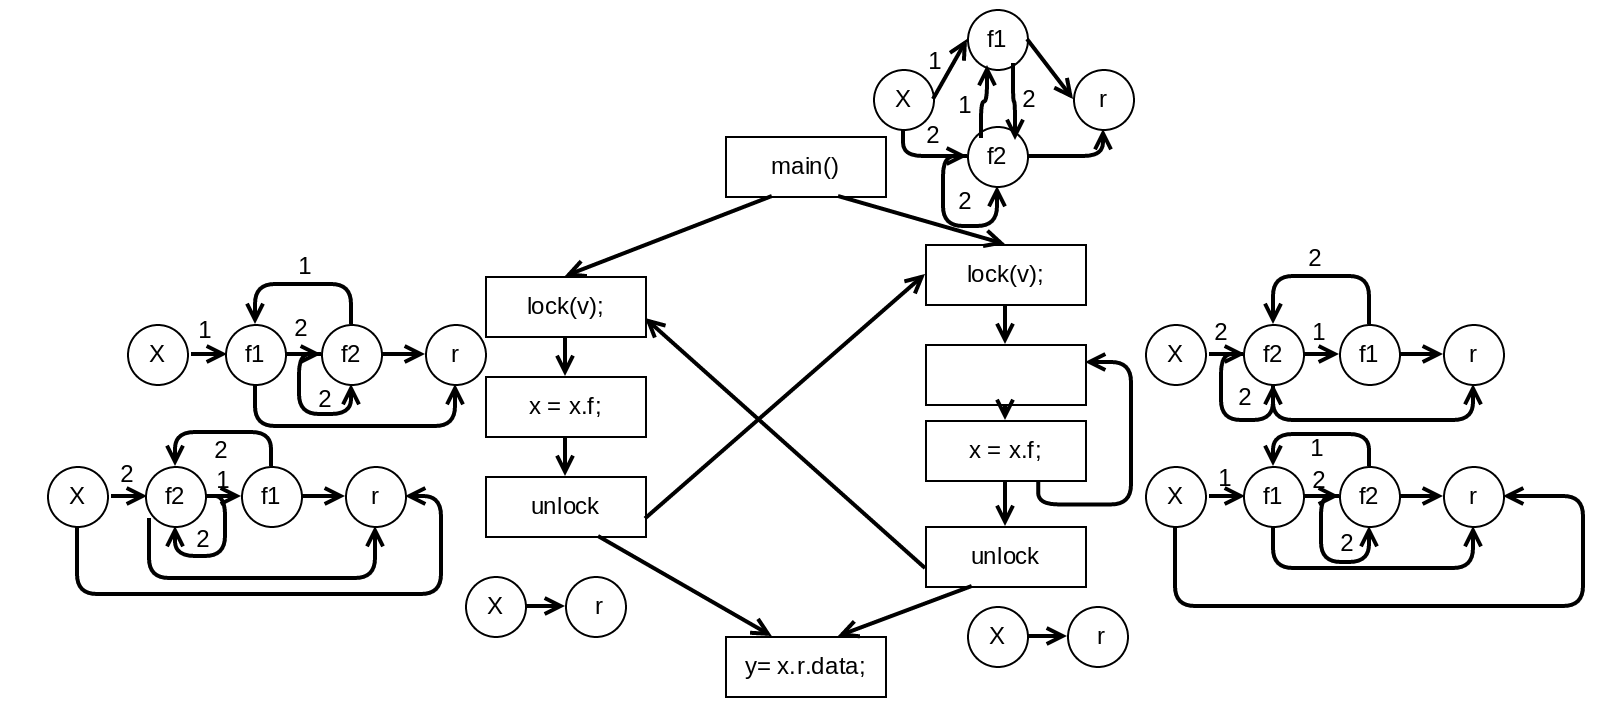
\includegraphics[width=0.8\textwidth]{Figures/rsz_loop_inside.png}
	\caption{Concurrent Heap liveness analysis example (on sync cfg). Note that edges in access graphs are marked by thread id}
	\label{fig:threadidanalysis}
\end{figure}

Another interesting case is when we have a loop across a critical section. This means that we can access the critical section zero or more times. In the previous 2 examples, we could only execute the critical sections once for all the threads. Consider the example shown in Figure 5.4. This is a slight modification of figure 5.3, with the loop being outside/across the lock/unlock statements. Even in this case applying the simple analysis on the program graph generated by adding the thread sync edges results in the same access graphs as the case of execution of loop inside  a critical section. \\

\begin{figure}
	\centering
	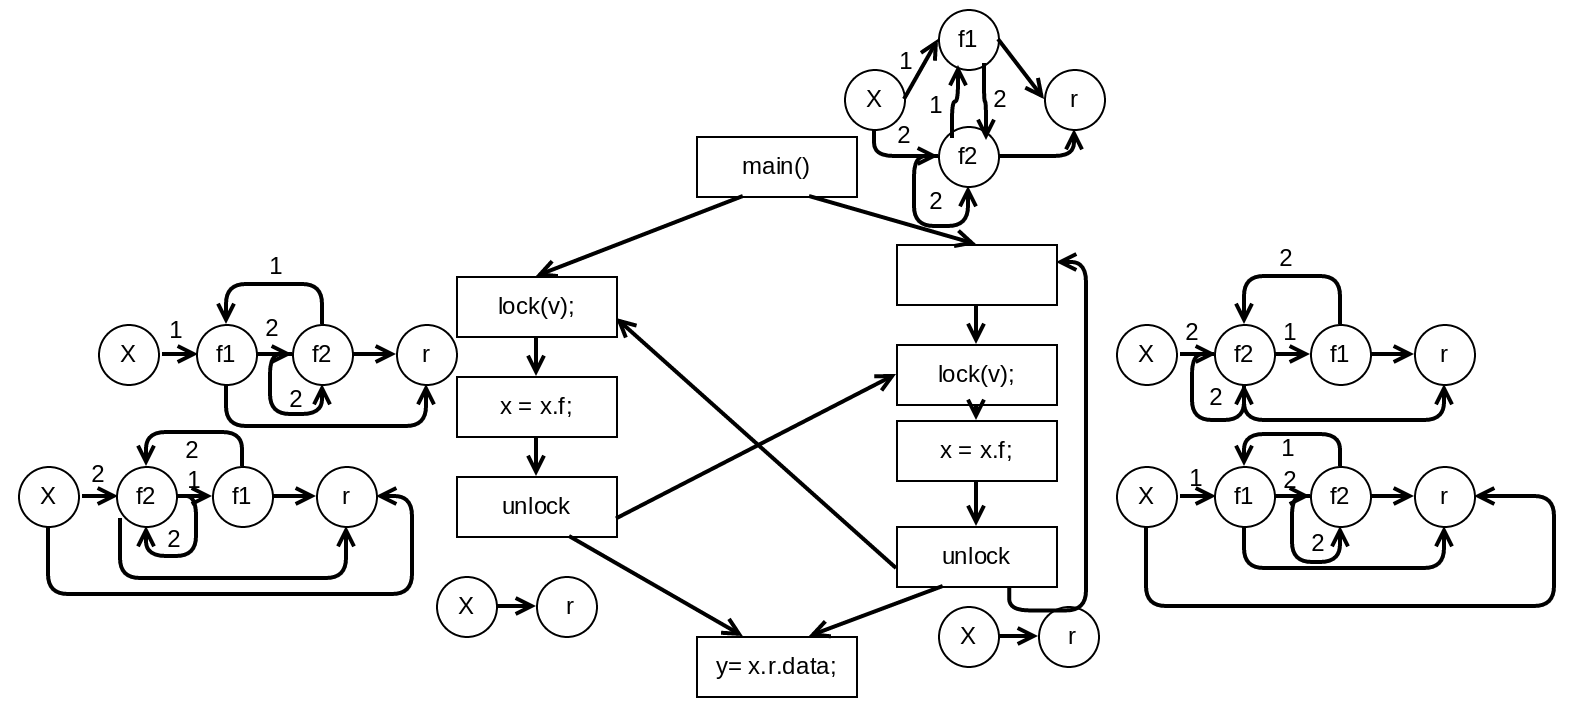
\includegraphics[width=0.8\textwidth]{Figures/rsz_loop_outside.png}
	\caption{Concurrent Heap liveness analysis example (on sync-cfg).}
	\label{fig:threadidanalysis}
\end{figure}

Clearly the two examples have different executions possible. But the access graph obtained from the analysis on program graph(sync-cfg generated by adding synchronization edges) leads to a highly approximated access graph. Also there is no difference between the access graphs. The possible live access links at the program point main() are \emph{$x$.$f_1$.$f_2$\textsuperscript{*}} and \emph{$x$.$f_2$\textsuperscript{+}.$f_1$.$f_2$\textsuperscript{*}} for the example in figure 5.4. Example 5.4 is also different from 5.3 in a way that, the critical section of $thread_2$ in 5.4 can itself be executed zero or more times. Whereas in the case of 5.3, it would have only been executed once. \\

Summarizing all the problems we have encountered with the analysis technique. The first one being treatment of synchronization edges of the program graph same as other edges. This leads to formation of loop in the control flow graph. During propagation of data flow values in the analysis, the values are transferred in the loop until a stable/converged value is reached. This fact corresponds to execution of the critical section(s) multiple times, which may not be the case most of the times. We would need to look at the analysis from the point of view of concurrent program execution. This analysis just assumes any starting point and merges data flow value along all the executions. In order to improve upon the precision we would need to come up with different starting points corresponding to each thread and propagate data flow values taking each thread as the starting point. Also , we would need to come up with a way to ensure that facts are propagated according the number of critical section executions possible.           